\section{Introduction}
% add citations to cms ot upgrade and lhc upgrade 
The Phase-2 CMS silicon tracker upgrade \cite{CMSouterTrackerPh2TDR} will have to provide high-quality physics data while operating at the extreme beam intensities and particle collision rates foreseen at the high-luminosity upgrade of the Large Hadron Collider (HL-LHC). The outer tracker (OT) will be built from double-layered modules, each consisting of two strip (2S), or one pixel and one strip (PS) silicon sensors.
% The 2S modules in the outermost three layers (radii greater than 600mm). 
% add reference to TDR again for the module drawing 
\begin{figure}[!htbp]
\centering
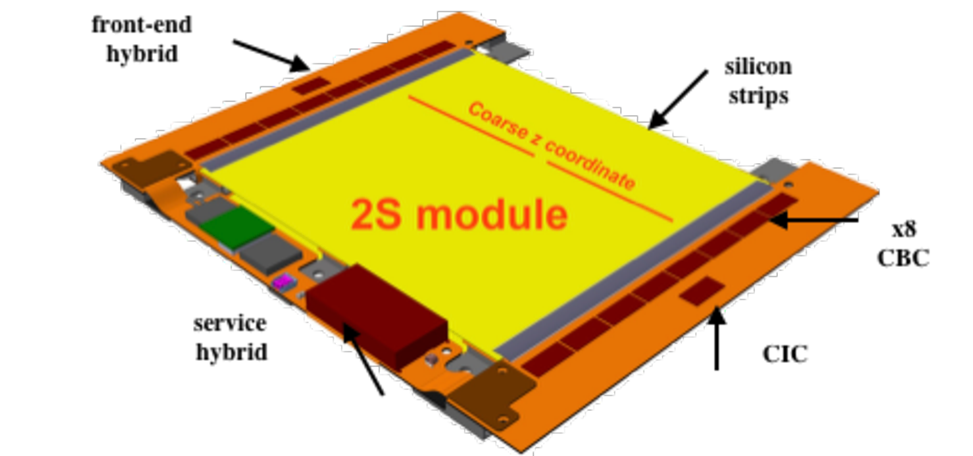
\includegraphics[width=0.75\linewidth]{Figures/Drawing_2Smodule.pdf}
\vspace*{-2mm}
\caption[2S module.]{An OT 2S module with two front-end hybrids containing sixteen CBC3s for read out the full module. A service hybrid will provide power and data connectivity.} 
\label{fig:Schematic2Smodule}
\end{figure} 

A single module can identify high transverse momentum tracks by looking for a pair of coincident hits (a stub) in nearby channels in the two closely separated sensors. Stubs from different layers can then be combined into tracks in off-detector electronics. The CMS Binary Chip (CBC) is a 254-channel front-end ASIC manufactured in 130 nm CMOS technology for the readout of the 2S modules (shown in \cref{fig:Schematic2Smodule}). The CBC3 \cite{CBC3} is the final prototype of the ASIC and the first to include the full logic circuitry required for stub finding.



% probably can live without this bit...
% % JG - stripped it down a bit, need to add reference
% % S.S - trying without this bit (! no space!! ) 
% The CBC generates a binary value for each connected strip to indicate whether the measured charge exceeded a set threshold (Vth in Figure.\cref{fig:CBC3}). The input channels are connected alternately to the strips on the two sensor layers; thus enabling the stub finding circuitry to search for correlated hits in the two layers within a programmable correlation window. 

% The location and directional data for all identified stubs, along with error and synchronization bits, are shared across five differential Scalable Low-Voltage Signaling (SLVS) pads and output from the CBC3 at a rate of $320$\MHz. 
% cite Kirika's Hiroshima paper/ M.Pedyyrech's TWEPP paper 
% \begin{figure}[htbp]
% \centering
% 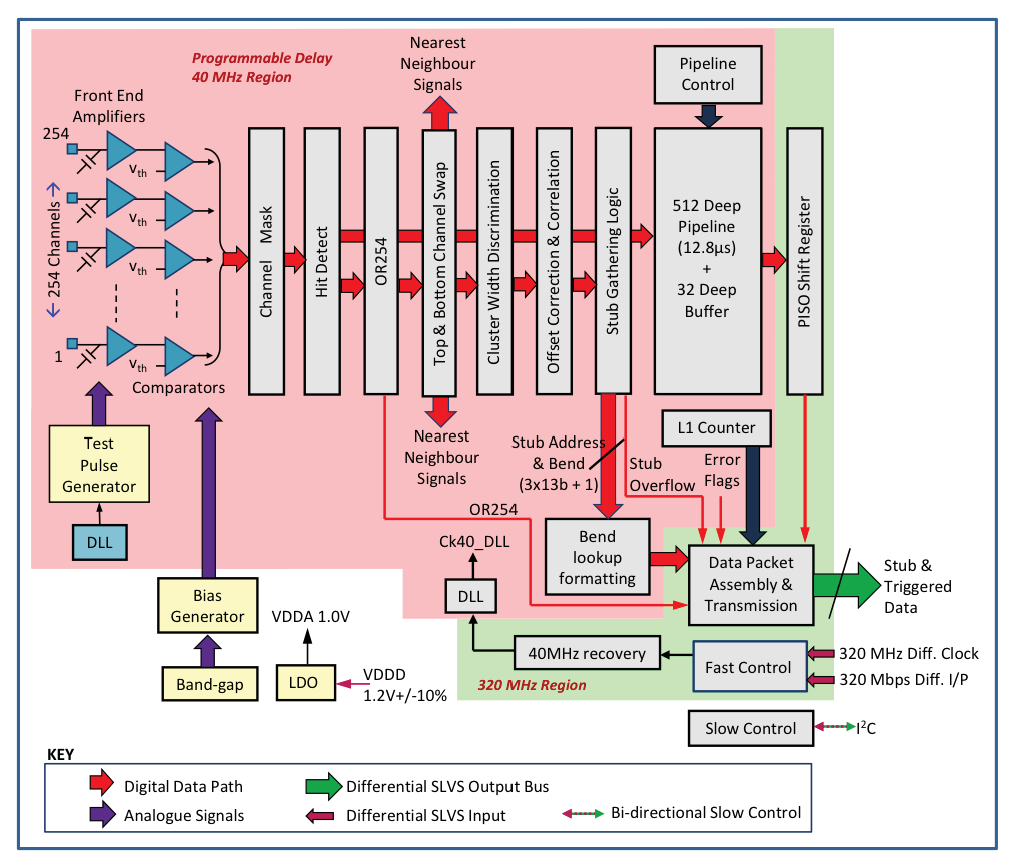
\includegraphics[width=0.9\linewidth]{Figures/Architecture_CBC3.eps}
%  \caption[Architecture of CBC3.]{A simplified block diagram describing the architecture of the CBC3: data from up to a maximum of 512 bunch crossings can be stored on-chip to allow time for the L1 trigger system to decide which event data should be read out for further processing.}
%  \label{fig:Architecture_CBC3}
% \end{figure} 

% Drop these figures if you're running out of space
\begin{figure}[!htbp]
\centering
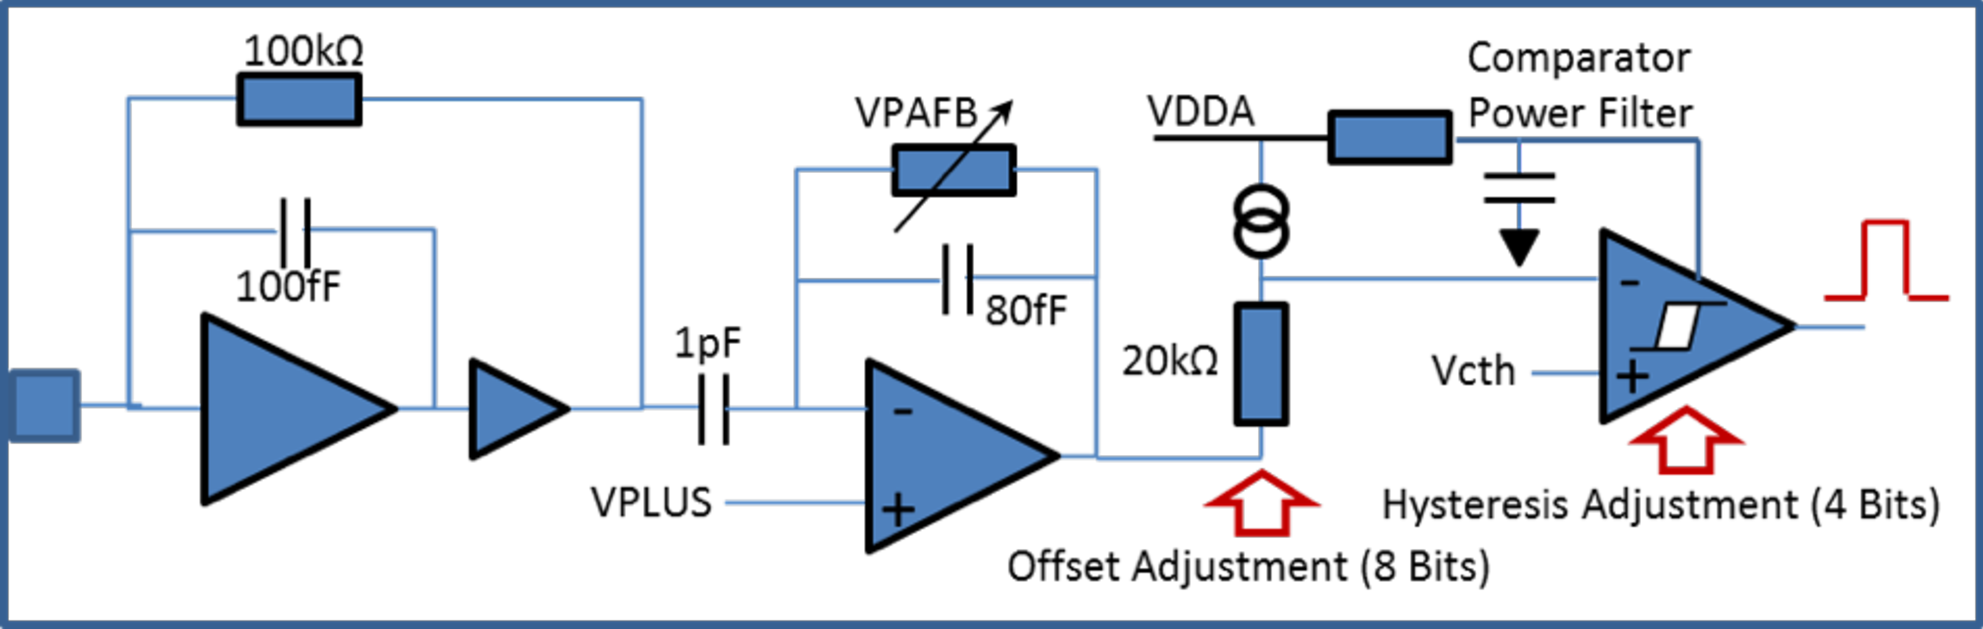
\includegraphics[width=0.9\linewidth]{Figures/Architecture_AnalogueFE}
\vspace*{-2mm}
\caption[Fit.]{A schematic of the CBC3 analogue front-end.}
\label{fig:Architecture_AnalogueFE}
\end{figure} 
% \begin{figure}[!htbp]
% \centering
% 	\subfloat[][The architecture of the CBC3.]
%   {
%     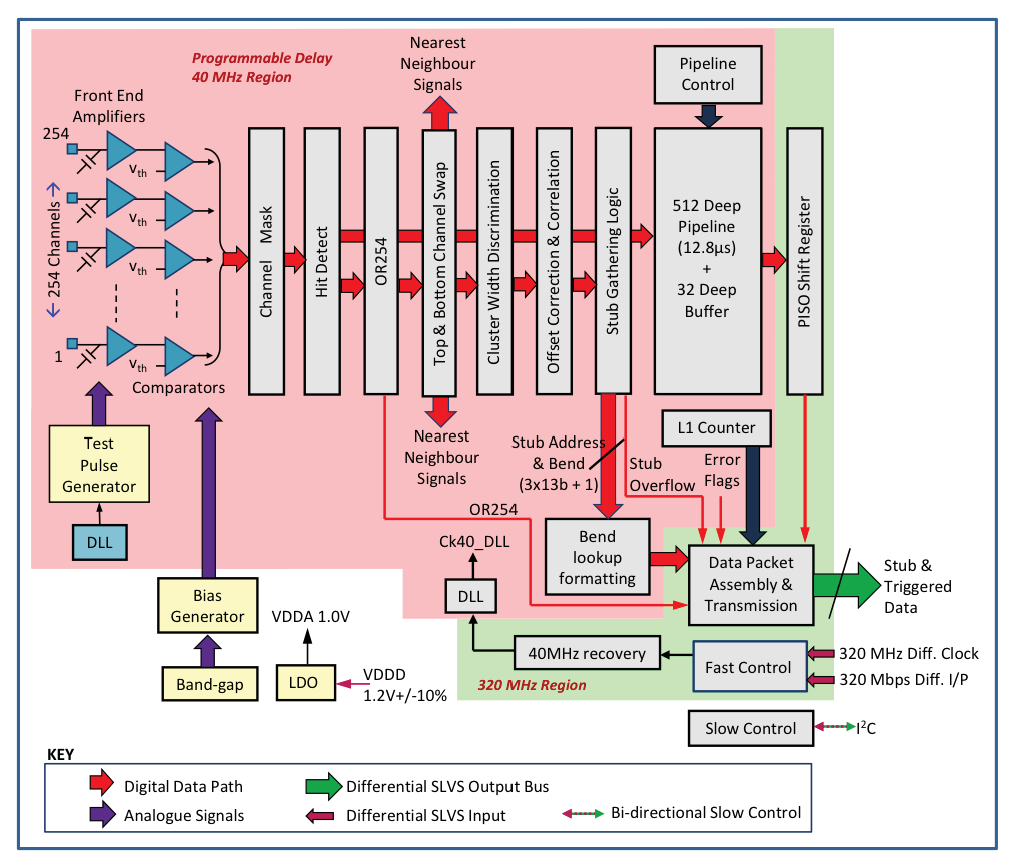
\includegraphics[width=0.9\linewidth]{Figures/Architecture_CBC3.eps}
%     \label{fig:Architecture_CBC3}
%   }
%   \quad
%   \subfloat[][Schematic of the CBC3's analogue front-end.]
%   {
%     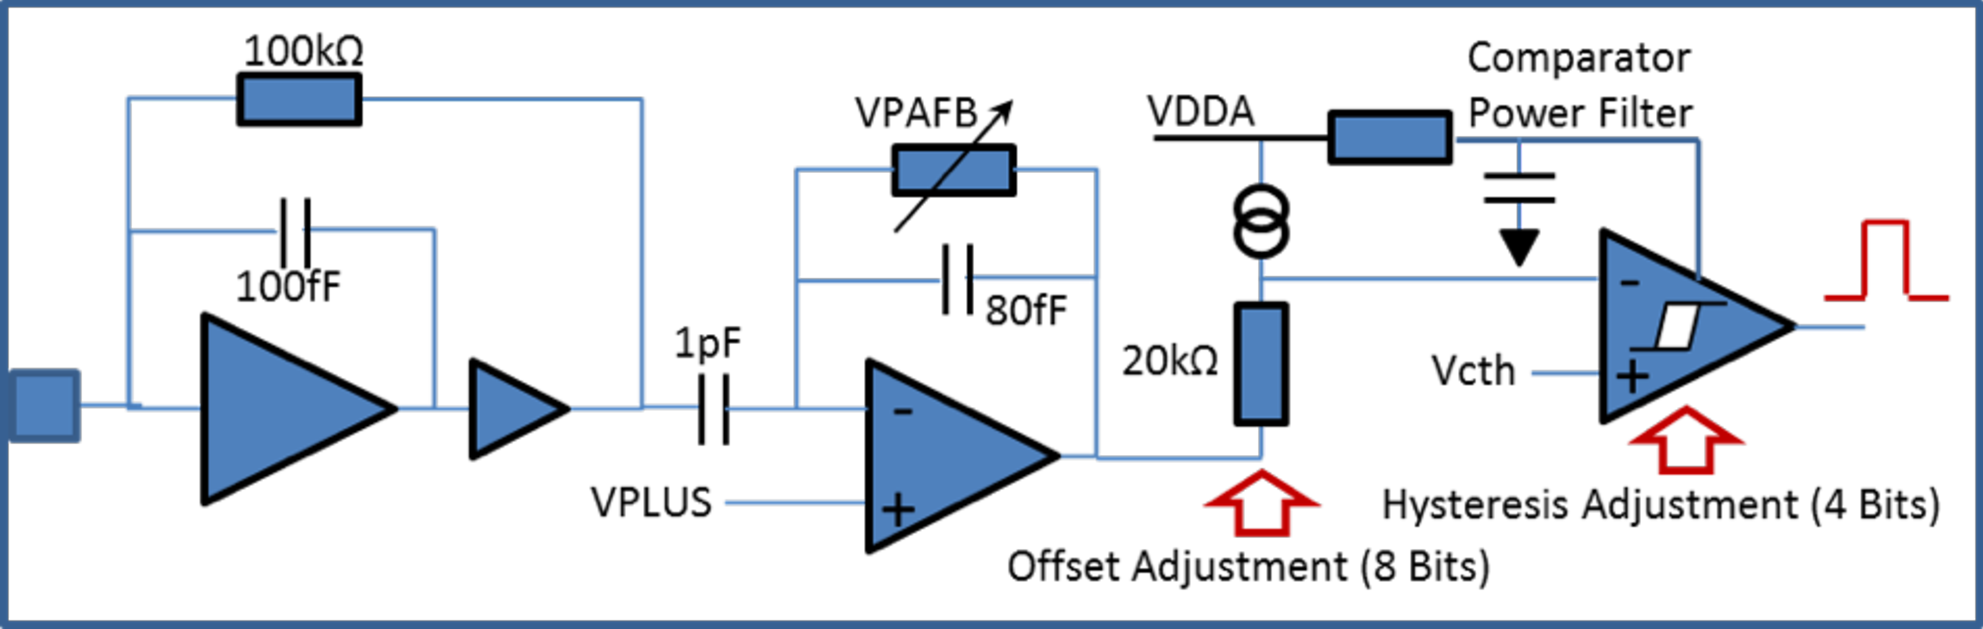
\includegraphics[width=0.9\linewidth]{Figures/Architecture_AnalogueFE}
%     \label{fig:Architecture_AnalogueFE}
%   }
%   \caption[Fit.]{Simplified block diagrams describing the architecture of the CBC3 and its analogue front-end.}
%   \label{fig:CBC3}
% \end{figure} 
 
%reference to CBC2 radiation testing (BragaThesis)
Total ionizing dose (TID) tests performed on the previous prototype \cite{CBC2nim} of the CBC showed a large, but temporary, increase in digital current and a pipeline sensitivity to occupancy. Both effects were attributed to radiation-induced leakage in the SRAM elements of the pipeline which motivated the decision to modify the SRAM block in the CBC3. 
% The NMOS read- and write-access transistors in the SRAM block were replaced with more radiation-resistant PMOS devices, and the NMOS pull-down transistors of the SRAM cross-coupled inverters were replaced with more radiation-resistant enclosed layout (ELT) NMOS devices. 

In this report the results of an X-ray irradiation campaign measuring the radiation-tolerance of the CBC3 are reported. A radiation damage model, developed to extrapolate the results to HL-LHC operating conditions, will also be described.